\documentclass[main.tex]{subfiles}
\begin{document}

\subsection{Wall Collision}

The purpose of this component is two-fold, firstly to give the dead-reckoning system a sense of walls and the limits they enforce on movement. Secondly to ensure that any error from not taking into account walls is not introduced. The basic concept is that when the application believes the user has taken a step in a given direction, it verifies that step can logically be taken. For example if a step is detected and user is facing a wall, the system should not believe that the user has moved through a wall.

\subsubsection{Initial Implementation}

For the initial implementation the extracted floor plan graphs are used as the basis for deciding whether a step the systems believes the user has made is valid or not. These graphs have one important feature that allows for this, two adjacent nodes are not connected if there is a wall between the corresponding positions in the floor plans. This allows for the following procedure to determine if a step is valid:

\begin{itemize}
	\item \textbf{Assign the nearest node to the user} - The node nearest to the user's estimated real position is assigned to the user, this can be used for path finding a new route if required, or in this case determing the validity of a movement. The nearest node was originally found through a brute force search, this was later changed utilising the search functions in-built to the graph packages, as it was faster.
	\item \textbf{Simulate a step} - A step is then simulated from the user's real position, this is essentially calculating where the user will move to given their current heading and rough stride length estimate. The stride length was initially set to the equivalent of 12 pixels in the floors plans, since the distance between nodes is 10 therefore allowing for proper testing. 
	\item \textbf{Check for new nearest node} - From the new simulated real position check if there is a new nearest node:
	\begin{itemize}
		\item If there is a new nearest node, path find from the first nearest node to the new one. If path length is greater than 2 you must have transitioned over a wall, see Figure~\ref{fig:iniCol} for an example. If the path length is less than or equal to 2 the move is valid
		\item If the nearest node doesn't change the move is valid
	\end{itemize}
\end{itemize}

\begin{center}
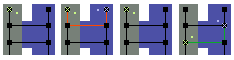
\includegraphics[scale=1.5]{images-implementation/collision1.png}
\captionof{figure}{Diagrams showing the above steps, the lefthand pair is a step by rejecting due to a path length of 3, the righthand pair accept the step as valid}
\label{fig:iniCol}
\end{center}

\subsubsection{Issues}

This implementation serves it's purpose but it was ultimately scrapped due to the following two reasons:

\begin{enumerate}
	\item The initial implementation is gated by the distance between two nodes. If the stride length is greater than two and a half times the number of pixels between nodes, then every step will have a path length greater than 3. Meaning every step is then rejected, the step length we found to be the average of our groups equated to around 30 pixels. This problem can be bypassed by simply running the method over 30 pixels in 3 chunks of 10.
	\item Due to the reliance on path finding it heavily slows down the application to unusable levels. This is exacerbated by the need to repeat it multiple times to work over the set stride length
\end{enumerate}

Whilst the first problem was fixable the second was not without creating a new method, the implementation below was made to solve this issue.

\subsubsection{Final Implementation}

With the initial method being too slow, another one was developed. Instead of working directly with the graph, which causes the slow down due to path finding, it works with the raw hand curated floor plan image. It directly looks at the colours of pixels within this image to determine if the path from start to end would have crossed a wall, a white pixel.

It does this by taking the co-ordinates of the current nearest node and the new nearest node from the simulated step and creating a path, pixel by pixel, between the two node locations. It decides whether to move in the X and Y by examining which of the difference in X or Y between the path's head and end point is larger. It selects the larger difference and then assesses which direction it needs to move by checking which co-ordinate of the two locations is larger. For example to move left the difference between path's X and end's X needs to be greater than the Y difference of these two points and then the path's X is greater than the end's X co-ordinate.

Once the next pixel in the path has been chosen in then checks the colour of that pixel, if it is white then the user's step will hit a wall and it returns the step is invalid. If the pixel is not white continue pathing between the nodes. This repeats pixel by pixel until the end location is reached and now the move is considered valid as no white pixels existed on the path.

This proved to be a much faster method and removed the lag that was being experienced with the previous method, the cost of loading the image is at the very start of the application.

\end{document}